
	\section{Produkteinsatz}

		\subsection{Beschreibung des Problembereichs}
		Der Problembereich lässt sich für diese Analysestufe in drei Punkte einteilen, um eine Gesamtkoordination effizient zu gestalten:

		\begin{enumerate}
		\item
			Zuallererst muss das automatische Fahren im zweidimensionalen
			Koordinatensystem zu einem angegebenen Zielpunkt(\emph{Destination})
			fehlerfrei möglich sein. Ebenfalls steht eine manuelle Steuerung zur
			Verfügung, um unerwarteten Ereignissen zu begegnen, die allerdings
			wiederum sinnvoll in das Gesamtsystem integriert werden muss.
		\item
			Als zweite Herausforderung geht es darum den Schaden von Kollisionen
			zu minimieren; wie diese erkannt, wie auf sie reagiert wird und diese
			Kollisionen durch vorrauschendes Umfahren von
			Objekten (\emph{Obstacle}) verhindert werden können. Dies schließt
			sowohl bewegliche Objekte als auch unbewegliche Objekte mit ein.
		\item
			Im dritten Punkt gilt es einen möglichst reibungs- und
			unterbrechungslosen Batteriebetrieb zu garantieren, um zeitlich
			vorrauschendes Fahren zu ermöglichen. Im Falle eines niedrigen
			Batteriestands also unverzüglich an seiner individuellen Ladestation
			(\emph{Charger}) anzudocken und aufzuladen, beziehungsweise längere
			Fahrten nicht anzutreten, die den Batteriestand gefährden würden.
		\end{enumerate}

		\begin{figure}[H]
			\centering
			\begin{subfigure}[t]{0.3\textwidth}
				\includegraphics[width=\textwidth]{../images/grafikZumProblembereich1.jpg}
				\caption{Fahren zu einem angegebenen Zielpunkt}
				\label{fig:2-1-problembereich-1}
			\end{subfigure}
			~~~~
			\begin{subfigure}[t]{0.3\textwidth}
				\includegraphics[width=\textwidth]{../images/grafikZumProblembereich2.jpg}
				\caption{Umfahren von Objekten}
				\label{fig:2-1-problembereich-2}
			\end{subfigure}
			~~~~
			\begin{subfigure}[t]{0.3\textwidth}
				\includegraphics[width=\textwidth]{../images/grafikZumProblembereich3.jpg}
				\caption{Automatisches Laden}
				\label{fig:2-1-problembereich-3}
			\end{subfigure}
			\caption{Visualisierung der Problembereiche}\label{fig:2-1-problembereiche}
		\end{figure}

		Abbildung \ref{fig:2-1-problembereiche} zeigt die drei o.g. Problembereiche in einer fotografischen Repräsentation.\\


		Daran anknüpfend wird mit folgenden Annahmen gearbeitet:

		\begin{enumerate}
		\item
			Zur Vereinfachung des Fahrverhalten muss jedes Zielobjekt physisch
			erreichbar sein. Ziele sind dementsprechend keine Hindernisse, das
			gleiche gilt für Ladestationen.
		\item
			Roboter können autark vom \emph{Server} agieren, damit ihre Ziele
			bestimmen und eine Ladestation anfahren.
		\item
			Bei den beweglichen Objekten wird davon ausgegangen, dass es sich im
			Verkehrsbetrieb ausschließlich um andere Roboter handelt. Für die
			unbeweglichen Objekte ist es notwendig, dass ihre Position von
			vornerein bekannt ist und sie unverändert bleibt.
		\end{enumerate}

		\subsection{Glossar}

		% \begin{description}
		% 	\item[Robot]{Roboter, der sich im 2-Dimensionalen Raum bewegen kann.}
		% 	\item[Server]{Verteilt Aufträge an die Roboter}
		% 	\item[Charger]{Ladestation für den Roboter}
		% 	\item[Destination]{Vom Server verwaltete Ziele, die der Roboter ansteuern kann.}
		% 	\item[Obstacle]{Hindernisse, die der Roboter erkennt und umfährt.}
		% \end{description}

			\begin{tabular}{ l p{10cm} }
		\textbf{Begriff} & \textbf{Erklärung}\\
		Robot & Roboter, der sich im 2-Dimensionalen Raum bewegen kann. Der wird
		als Fahrzeug verwendet und kann Personen transportieren.\\
		Position & Eine Position ist eine Zweidimmensionale Position im Raum,
		also ein Punkt, zu dem der Roboter fahren kann\\
		Task & Ein Task behinhaltet zusätzlich zu einer Position auch eine
		Geschwindigkeit. Fadurch kann der Server dem Roboter mitteilen, ob
		dieser vorsichtig oder schnell zu einer Position fahren
		soll.\\
		Server & Der serve ist eine einzelne, zentrale Instanz, die die Aufträge
		an die Roboter verteilt\\
		Charger & Ladestation für den Roboter\\
		Destination & Ziele die der Roboter ansteuern kann.\\
		Obstacle & Hindernisse, die der Roboter erkennt und umfährt Dies können
		entweder andere Roboter sein, mit denen der Roboter kommunizieren kann
		um eine Priorität festzulegen oder statische Hindernisse der
		Umgebung.\\
		Hospital & Das Krankenhaus, das mit dem System kommuniziert, um die Robots
		für Krankentransporte einzusetzen.
	\end{tabular}

		
		
		\subsection{Modell des Problembereichs}
		Abbildung \ref{fig:2-3-modell-problembereich} zeigt ein Klassendiagramm, welches das Modell des Problembereichs grafisch darstellt.
		\begin{figure}[H]
			\centering
			\includegraphics[width=0.8\textwidth]{../images/Problembereich.pdf}
			\caption{Klassendiagramm des Problembereichs}
			\label{fig:2-3-modell-problembereich}
		\end{figure}

		\subsection{Beschreibung der Geschäftsprozesse}

			\subsubsection*{Beschreibung zu 1: Choose Robot}

			\begin{table}[H]
				\centering
				\begin{tabularx}{\textwidth}{@{}p{3cm}X@{}}
				\toprule
				\textbf{Auslösendes Ereignis:} & Der Server will den für ein bestimmtes Ziel bestmöglichen Roboter auswählen und diesen zum Ziel schicken. \\ \midrule
				\textbf{Ergebnis:} & Alle Roboter haben ihre Sensordaten ausgelesen und diese dem Server
				mitgeteilt. Daraufhin hat der Server einen Roboter ausgewählt, der für
				die Zielanfahrung optimal geeignet ist, und diesem den Auftrag zum
				Anfahren des Ziels übermittelt. \\ \midrule
				\textbf{Mitwirkende:} &	Server, Roboter \\
				\bottomrule
				\end{tabularx}
				\label{tab:2-4-choose-robot}
			\end{table}

			Abbildung \ref{fig:2-4-choose-robot-aktivitaetendiagramm} zeigt ein Aktivitätendiagramm, welches den Ablauf des Geschäftsprozesses \emph{1: Choose Robot} darstellt.
			\begin{figure}[H]
				\centering
				\includegraphics[width=\textwidth]{img/1-Analyse-3-Choose_Robot}
				\caption{Illustration von \emph{1: Choose Robot} durch Aktivitätendiagramm}
				\label{fig:2-4-choose-robot-aktivitaetendiagramm}
			\end{figure}

			Um den für ein gegebenes Ziel bestmöglichen \emph{Robot} auszuwählen, sendet
			der \emph{Server} zunächst an alle \emph{Robots} eine Anfrage (\emph{request}),
			woraufhin die \emph{Robots} ihre Sensordaten (\emph{sensor data}) auslesen und
			an den \emph{Server} senden. Auf Grundlage dieser Daten wählt der \emph{Server} den
			\emph{Robot} aus, der für die Erfüllung des Zieles am besten geeignet ist. Es kann auch vorkommen, dass kein \emph{Robot} geeignet ist, um ein Ziel zu erfüllen. Wie die Sensordaten und der Algorithmus zur Wahl des optimalen \emph{Robots} konkret definiert sind, ist eine Entwurfsentscheidung.

			\subsubsection*{Beschreibung zu 2: Drive to Destination}

			\begin{table}[H]
				\centering
				\begin{tabularx}{\textwidth}{@{}p{3cm}X@{}}
				\toprule
				\textbf{Auslösendes Ereignis:} & Ein \emph{Robot} hat eine \emph{Destination} erhalten.\\ \midrule
				\textbf{Ergebnis:} & Der \emph{Robot} ist unter Umfahrung von womöglichen \emph{Obstacles} zur \emph{Destination} gefahren.\\ \midrule
				\textbf{Mitwirkende:} &	Ein einzelner, autonomer \emph{Robot}. \\
				\bottomrule
				\end{tabularx}
				\label{tab:2-4-drive-to-destination}
			\end{table}

			Abbildung \ref{fig:2-4-drive-to-destination-aktivitaetendiagramm} zeigt ein Aktivitätendiagramm, welches den Ablauf des Geschäftsprozesses \emph{2: Drive to Destination} darstellt.

			\begin{figure}[H]
				\centering
				\includegraphics[width=\textwidth]{../images/Iteration0_Analyse_2-4_driveToDestination}
				\caption{Illustration von \emph{2: Drive to Destination} durch Aktivitätendiagramm}
				\label{fig:2-4-drive-to-destination-aktivitaetendiagramm}
			\end{figure}

			Dieser Prozess wird autonom vom \emph{Robot} ausgeführt. Er wird genau
			dann ausgeführt, wenn der Roboter eine \emph{Destination} vom Server
			erhalten hat, die er anfahren soll. Da der \emph{Robot} an dieser Stelle
			dem Server schon bestätigt hat, dass sein Akkustand hoch genug ist, ist
			der einzige Sonderfall, den wir betrachten müssen, dass ein
			\emph{Obstacle} auf der direkten Linie zwischen \emph{Robot} und
			\emph{Destination} liegt. Dann wird der \emph{Robot} nach Wahl des
			besten Umweges das \emph{Obstacle} umfahren und wieder die Fahrt zur
			\emph{Destination} Aufnehmen.



			\subsubsection*{Beschreibung zu 3: Take Patient to Hospital}

			\begin{table}[H]
				\centering
				\begin{tabularx}{\textwidth}{@{}p{3cm}X@{}}
				\toprule
				\textbf{Auslösendes Ereignis:} & Das \emph{Hospital} hat einen neuen Patienten registriert.\\ \midrule
				\textbf{Ergebnis:} & Der Robot ist zum \emph{Patient} gefahren, dieser wurde von Helfenden auf den \emph{Robot} geladen 
				und der \emph{Robot} hat den \emph{Patient} zum \emph{Hospital} zurück gebracht.\\ \midrule
				\textbf{Mitwirkende:} &	Ein einzelner, autonomer \emph{Robot}, der \emph{Server} und das \emph{Hospital}. \\
				\bottomrule
				\end{tabularx}
				\label{tab:2-4-take-patient-to-hospital}
			\end{table}

			Abbildung \ref{fig:2-4-take-patient-to-hospital-aktivitaetendiagramm} zeigt ein Aktivitätendiagramm, welches den Ablauf des Geschäftsprozesses \emph{3: Take Patient to Hospital} darstellt.

			\begin{figure}[H]
				\centering
				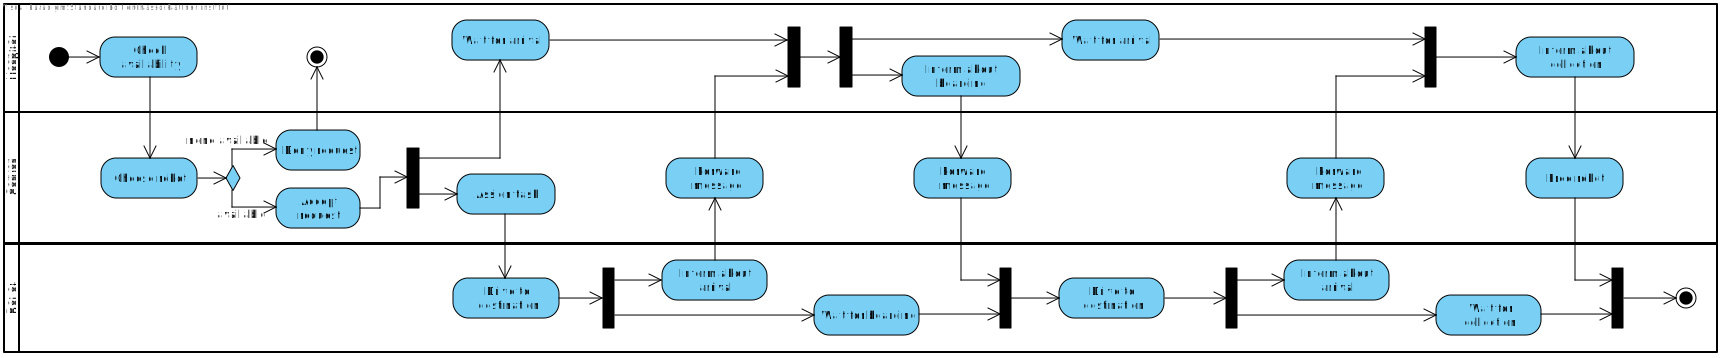
\includegraphics[width=\textwidth]{img/1-Analyse-2-Geschaeftsprozess_TakePatientToHospital}
				\caption{Illustration von \emph{3: Take Patient to Hospital} durch Aktivitätendiagramm}
				\label{fig:2-4-take-patient-to-hospital-aktivitaetendiagramm}
			\end{figure}

			Um die Verfügbarkeit eines \emph{Robots} anzufragen gibt das \emph{Hospital} die Adresse des \emph{Patient} an den \emph{Server}. Dieser wählt dann den passenden \emph{Robot} aus. Falls keiner verfügbar ist, lehnt der \emph{Server} den Krankentransport ab, anderenfalls wird dem \emph{Robot} dieser \emph{Task} zugewiesen. Darauf fährt der \emph{Robot} zum \emph{Patient}, wenn er angekommen ist, gibt er das über den \emph{Server} ans \emph{Krankenhaus} weiter und wartet bis die Helfenden den \emph{Patient} aufgeladen haben. Nach dem Aufladen informiert das \emph{Hospital} den \emph{Robot} und wartet selber bis der \emph{Patient} am \emph{Hospital} angekommen ist. Darauf fährt der \emph{Robot} zum \emph{Hospital} und wartet bis der \emph{Patient} abgeladen ist. Danach ist er wieder für alle weiteren \emph{Tasks} verfügbar.

	\pagebreak

	
